% Kinematika částice
%---------------------------------------------------------------------------------------------------
% file kinematika.tex
%---------------------------------------------------------------------------------------------------
\chapter{Kinematika částice}
\minitoc
\newpage
  Nejjednodušší fyzikální soustava je jeden hmotný bod, který se pohybuje v prostoru a čase. Pojem
  hmotný bod je ovšem abstrakce, model, kterým nahrazujeme reálnou částici. Vyjadřujeme jím, že
  odhlížíme od tvaru a rozměru částice, považujeme ji za bodovou, a kromě její geometrické polohy v
  daném okamžiku jí připisujeme pouze jedinou fyzikální vlastnost, hmotnost. V tomto smyslu budeme
  v mechanice často místo hmotného bodu hovořit prostě o částici.
  %----------------- Kinematický popis pohybu částice ---------------------------------------------- 
  \section{Kinematický popis pohybu částice}
    V kinematice se zajímáme pouze o průběh pohybu částice v prostoru a čase a nepátráme po
    příčinách tohoto pohybu a jeho změn. Předpokládáme, že částice se pohybuje po spojité křivce,
    trajektorii, a snažíme se určit jednak tvar této trajektorie a zákon pohybu po ní, tj. polohu
    částice na trajektorii v závislosti na čase\footnote{Představa o pohybu částice po trajektorii
    jako po spojité křivce vyplývá z naší smyslové zkušenosti. Ukazuje se, že v mikrosvětě tato
    představa neodpovídá skutečnosti a pojem trajektorie tam ztrácí smysl. Částice se v mikrosvětě
    pohybuje podle zákonu kvantové mechaniky a v daném okamžiku není možné současné přesně stanovit
    její polohu a rychlost}. Spojitá křivka má v každém bodě tečnu a můžeme zavést pojem okamžité
    rychlosti částice mířící ve směru této tečny.
  
    \begin{figure}[ht!]
      \centering
      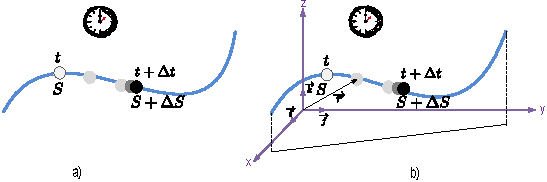
\includegraphics[width=\linewidth]{trajectory.pdf}
      \caption{Příklad trajektorie částice a zavedení kartézské soustavy souřadnic}
      \label{mech:fig_trjctr}
    \end{figure}
  
    Předpokládejme nejprve, že trajektorie částice je zadána. Pak můžeme od zvoleného bodu na
    trajektorii a zvoleného okamžiku měřit dráhu částice $s(t)$, tedy délku křivky, kterou částice
    za určitou dobu prošla (obr. \ref{mech:fig_trjctr}). V okamžiku $t$ je částice v bodě daném
    prošlou dráhou $s$, v okamžiku $t + \Delta t$ v bodě $s + \Delta s$. Dráha $s$ tu vlastně
    představuje parametr udávající polohu bodu na křivce; tímto způsobem popisujeme například pohyb
    automobilu na dálnici a udáváme na kterém je právě kilometru.
  
    Přitom můžeme zavést \textbf{střední rychlost částice} v intervalu $\Delta t$
    \begin{equation}\label{mech:eq_stredni_rychlost}
      \langle v\rangle=\frac{\Delta s}{\Delta t},
    \end{equation}
    \textbf{okamžitou rychlost částice} v okamžiku $t$
    \begin{equation}\label{mech:eq_okamzita_rychlost}
      v(t)=\lim_{\Delta t\rightarrow0}\frac{\Delta s}{\Delta t}=\frac{ds}{dt}=\dot{s}
    \end{equation}
    a \textbf{okamžité zrychlení}
    \begin{equation}\label{mech:eq_okamzite_zrychleni}
      a(t)=\lim_{\Delta t\rightarrow0}\frac{\Delta v}{\Delta t}
          =\frac{dv}{dt}=\lim_{\Delta t\rightarrow0}\frac{d^2s}{dt^2}=\dot{v}=\ddot{s}
    \end{equation}
    Takto zavedené rychlost a zrychlení jsou skalární funkce času a udávají pouze jak se mění dráha
    a rychlost při pohybu po zadané trajektorii, ve směru tečny k této trajektorii.
  
    Obecně však musíme udat polohu částice v prostoru vzhledem k nějaké vztažné soustavě. Tato
    soustava, například kartézská, je spojena s nějakým tuhým tělesem a doplněna hodinami
    umístěnými   například v počátku. V místnosti mohou jako kartézské osy sloužit průsečnice stěn
    a podlahy. Potom udáváme tři kartézské souřadnice částice jako funkce času:
    \begin{equation}\label{mech:eq_xyz}
      x=x(t),\quad y=y(t),\quad z=z(t)
    \end{equation}
    Soustava tří rovnic (rov. \ref{mech:eq_xyz}) představuje parametrické vyjádření tvaru
    trajektorie. Rovnici trajektorie v kartézských souřadnicích dostaneme, vyloučíme-li z rov.
    \ref{mech:eq_xyz} čas. Parametrem pohybu může být ovšem i dráha:
    \begin{equation}\label{mech:eq_draha}
      x = x(s),\quad y = y(s),\quad z = z(s).
    \end{equation}
    Přitom $s = s[x(t), y(t), z(t)]$ vystupuje jako složená funkce času. Výše zavedená skalární
    rychlost bude
  
    %-------------------------- Základní pohyby a jejich skládání---------------------------------------------
    \subsection{Základní pohyby a jejich skládání}
      Uvedeme nyní některé základní typy pohybu částice.
      \subsubsection{Pohyb přímočarý}
          Nechť přímočarý pohyb probíhá podél osy x s počátečními podmínkami $x = x_0,v_x =
          \dot{x}=v_{0_x}$ při $t = t_0$. Pak rozlišujeme
          \begin{itemize}
            \item \emph{Pohyb rovnoměrný} s konstantní rychlostí $v_{0_x}$ a nulovým zrychlením
                  $a_x=0$. Integrací a použitím počátečních podmínek dostáváme zákon pohybu:
                  \begin{equation}\label{mech:eq_primocar_rovnomer}
                    x=x_0+v_{0_x}(t-t_0)
                  \end{equation}
            \item \emph{Pohyb rovnoměrně zrychlený} s konstantním zrychlením $a_{0_x}$ kladným nebo
                  záporným. Integrací a použitím počátečních podmínek dostáváme zákon ry\-chlo\-sti a
                  zákon pohybu:
                  \begin{align}
                    v &= v_0x+a_0x(t-t_0), \\
                    x &= x_0+v_{0_x}(t-t_0)+\frac{1}{2}a_{0_x}(t-t_0)^2 \label{mech:eq_const_acc}.
                  \end{align}
                  Je-li při $t = 0 x = 0, v = 0$ dostaneme známé vztahy $$v=a_{0_x}t,\quad
                  x=\frac{1}{2}a_{0_x}t$$
            \item \emph{Pohyb nerovnoměrný} se zrychlením obecně závislým na čase $a(t)$. Pak
                  do\-sta\-ne\-me zákon rychlosti a zákon pohybu integrováním
                  \begin{align}
                    v &= v_{0_x}+\int_{t_0}^{t}{a(t)dt} \\
                    x &= x_0+v_{0_x}(t-t_0)+\int_{t_0}^{t}{v(t)dt}
                  \end{align}
          \end{itemize}
      \subsubsection{Pohyb kruhový}
      \subsubsection{Pohyb harmonický}
        Pohyb harmonický dostaneme jako projekci rovnoměrného kruhového pohybu kolem počátku do
        jedné z kartézských os. Například v ose $y$ pak máme
        \begin{equation}\label{mech:eq_p_harmon}
          y(t)=A\sin(\omega t+\varphi_0)
        \end{equation}
        kde 
        \begin{labeling}{$\omega t+\varphi_0$}
          \setlength{\itemindent}{2cm}
          \item[\(y\)]                     \(\ldots\)\emph{výchylka (elongace)}, 
          \item[\(A\)]                     \(\ldots\)\emph{amplituda}, 
          \item[\(\omega\)]                \(\ldots\)\emph{úhlová rychlost} $[rad\cdot s^{-1}]$,
          \item[\(T=\frac{2\pi}{\omega}\)] \(\ldots\)\emph{perioda} $[s]$, 
          \item[\(f=\frac{1}{T}\)]         \(\ldots\)\emph{frekvence} $[Hz]$, 
          \item[\(\omega t+\varphi_0\)]    \(\ldots\)\emph{fáze}, 
          \item[\(\varphi_0\)]             \(\ldots\)\emph{počáteční fáze při} $t=0$ neboli
                                                     \emph{fázová konstanta}.
        \end{labeling}
  
        Souřadnice vektorů rychlosti a zrychlení při harmonickém pohybu jsou
        \begin{subequations}
          \label{mech:eq_harm} 
          \begin{align}
            v_y = \dot{y} 
              & = \omega A\cos(\omega t+\varphi_0 )=
                  \omega A\sin(\omega t+\varphi_0+\frac{\pi}{2}), \label{mech:eq_harm_vy}         \\
             a_y = \ddot{y} 
              &= -\omega^2A\sin(\omega t+\varphi_0 )=
                  \omega^2A\sin(\omega t+\varphi_0+\pi).          \label{mech:eq_harm_ay}
          \end{align}
        \end{subequations}  
        Z těchto vztahů je vidět, že při harmonickém pohybu rychlost předbíhá výchylku o
        $\frac{\pi}{2}$ a zrychlení o $\pi$ (je v protifázi).

    %----------------- Skládání pohybů -------------------------------------------------------------
    \subsection{Skládání pohybů}
      Ačkoliv částice může konat současně několik pohybů, lze je vektorově skládat. Tento netriviální 
      poznatek usnadňuje studium mechanických pohybů. Ukážeme nyní některé zajímavé případy skládání pohybu.
  
    \subsubsection{Skládání kolmých přímočarých pohybů}
      Se skládáním kolmých přímočarých pohybů se setkáváme při \emph{vrhu těles v homogenním tíhovém poli ve 
      vakuu}. Uvažujme rovinný pohyb v rovině $x, z,$ při čemž v záporném směru osy $z$ má pohyb zrychlení 
      velikosti $g$.

      \begin{example}Výstřel z děla (ve vakuu).
        Dělová koule opouští hlaveň zadanou rychlostí. Určete:
        \begin{itemize}\addtolength{\itemsep}{-0.5\baselineskip}
          \item maximální dostřel pro zadanou úsťovou rychlost,
          \item hranice oblasti, ve kterém lze zasáhnout cíl,
          \item stanovte velikost potřebného náměru děla pro zasažení libovolného cíle uvnitř
                ochranné paraboly.
        \end{itemize}
        \begin{figure}[ht!]
          \centering
          \begin{tabular}{c}
            \subfloat[ ]{\label{mech:fig_delo1}
               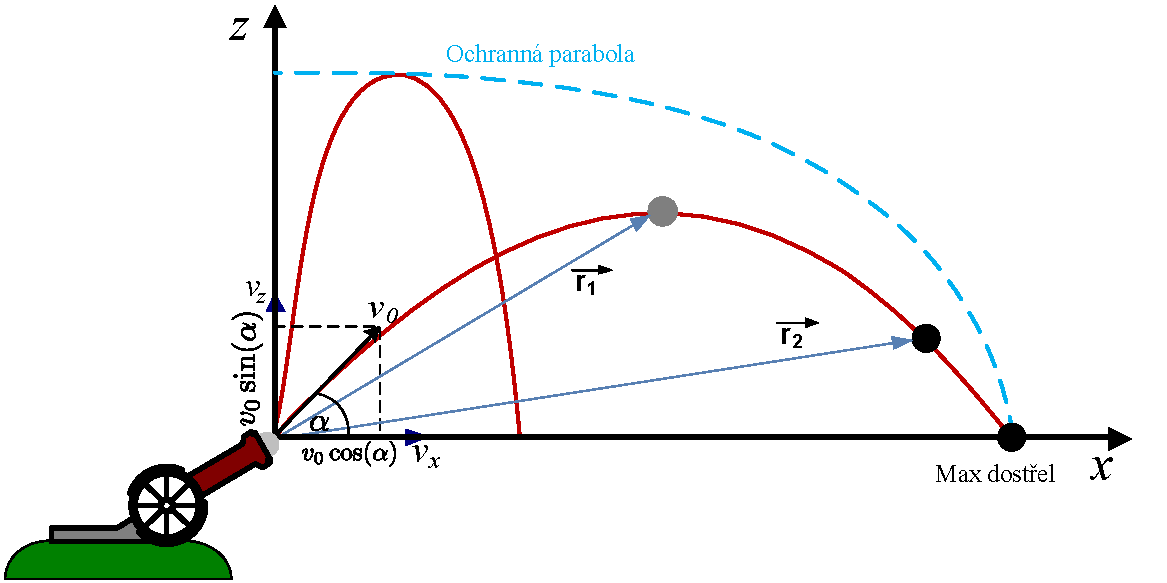
\includegraphics[width=0.9\linewidth]{kinematika_delo_vakuum.pdf}}      \\
            \subfloat[ ]{\label{mech:fig_tan_alpha}   
               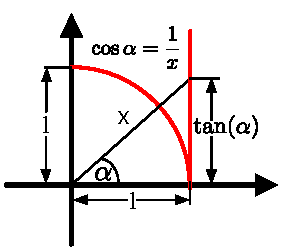
\includegraphics[width=0.3\linewidth]{kinematika_delo_tan_alpha.pdf}}
          \end{tabular}   
          \caption{K příkladu výpočtu trajektorie projektilu. Goniometrický vzorec
                   $|\cos\alpha|=\frac{1}{\sqrt{1+\tan\alpha^2}}$ lze snadno odvodit z náčrtu
                   pomocí Pythagorovy věty (Přepona pravoúhlého trojúhelníka je
                   $\sqrt{1+\tan\alpha^2}$)}            
        \end{figure}
        \textbf{Řešení:}
          Uvažujte rovinný pohyb v rovině $xz$, při čemž v záporném směru osy $z$ má pohyb zrychlení 
          velikosti $g$. Ve směru osy $z$ tedy probíhá rovnoměrně zrychlený pohyb podle rov. 
          \ref{mech:eq_const_acc}. Vztáhneme-li počáteční podmínky k okamžiku \(t = 0\), máme
          \begin{equation}\label{mech_eq_delo_vakuum_osa_z}
            z(t)=z_0+v_{0z}t-\frac{1}{2}gt^2, \qquad v_z(t)=v_{0z}-gt
          \end{equation}
          Ve směru osy $x$ je pohyb rovnoměrný:
          \begin{equation}\label{mech_eq_delo_vakuum_osa_x}
            x(t)=x_0+v_{0x} t,\qquad v_x(t)=v_{0x}=\mathrm{konst}
          \end{equation}

          Dělová koule opouští hlaveň pod elevačním úhlem $\alpha$ za podmínek dle obr.
          \ref{mech:fig_delo1} platí  $x_0=0, z_0=0, v_{0x}=v_0\cos\alpha>0,
          v_{0z}=v_0\sin\alpha>0$. Jde tedy o skládání \emph{rovnoměrného přímočarého pohybu s
          rychlostí} $v_0\cos\alpha$ ve směru osy $x$ a svislého pohybu vzhůru. Získané rovnice
          \begin{equation}\label{mech:eq_delo_rce_pohybu}
            z(t)=v_{0z}t-\frac{1}{2}gt^2, \qquad x(t)=v_{0x}t
          \end{equation}
          představují \emph{parametrické rovnice trajektorie}. Vyloučíme-li z nich čas $t$,
          dostaneme rovnici křivky v kartézských souřadnicích
          \begin{equation}\label{mech:eq_delo_vakuum_param_rce}
            z(x)=  \frac{v_{0z}}{v_{0x}}x-\frac{1}{2}\frac{g}{v_{0x}^2}x^2
                = x\tan\alpha-\frac{1}{2}\frac{g}{v_0^2\cos^2\alpha}x^2
          \end{equation}
          Nyní aplikujeme goniometrický vzorec
          \begin{equation*}
            |cos\alpha|=   \frac{1}{\sqrt{1+\tan^2\alpha}}\Rightarrow \frac{1}{\cos^2\alpha} 
                       = 1+\tan^2\alpha
          \end{equation*}
          odvozený dle náčrtku na obrázku \ref{mech:fig_tan_alpha} a dostáváme rovnici
          \begin{equation}\label{mech_eq_example_vysledna_rce}
            z(x)=x\tan\alpha-\frac{1}{2}\frac{g}{v_0^2}(1+\tan^2\alpha)x^2
          \end{equation}
          Pohyb projektilu (dělové koule) probíhá po stejné trajektorii, jako šikmý vrh v
          homogenním tíhovém poli ve vakuu, tedy po parabole. Snadno dostaneme \emph{souřadnice
          vrcholu dráhy, dálku doletu a celkovou dobu letu}.

          \begin{itemize}
            \item Maximální dolet pro daný elevační úhel:
              \begin{equation}\label{mech:eq_elevacni_uhel_1}
                0=x\tan\alpha-\frac{1}{2}\frac{g}{v_0^2}(1+\tan^2\alpha)x^2
              \end{equation}
              \emph{Netriviální kořen této kvadratické rovnice je námi hledaný dolet dělové koule}
              \begin{equation}\label{mech:eq_elevacni_uhel_2}
                x_d=\frac{2v_0^2\tan\alpha}{g(1+\tan^2\alpha)}(1+\tan^2\alpha)
                   =\frac{2v_0^2\sin\alpha\cos\alpha}{g}=\frac{v_0^2\sin{2\alpha}}{g}
              \end{equation}

            \item Celková doba letu:
              \begin{equation}\label{mech:eq_doba_letu}
                t_d=\frac{x_d}{v_{0x}} =\frac{2v_0^2\sin\alpha\cos\alpha}{gv_0\cos\alpha}
                   =\frac{2v_0\sin\alpha}{g}
              \end{equation}

            \item Souřadnice vrcholu dráhy: \emph{získáme derivováním rov.
                  \ref{mech_eq_example_vysledna_rce}}
                  \begin{align}
                    0   &= tan\alpha-\frac{g}{v_0^2(1+\tan^2\alpha)}x_v                         \\
                    x_v &= \frac{v_0^2}{g}\frac{\tan\alpha}{1+\tan^2\alpha}=
                           \frac{v_0^2}{g}\frac{\sin\alpha}{\cos\alpha}
                           \cdot\cos^2\alpha\cdot\frac{2}{2}                                   \\
                    x_v &= \frac{v_0^2\sin{2\alpha}}{2g}
                   \end{align}
                   \emph{Souřadnici $z_v$ dostaneme dosazením $x_v$  do rov.
                   \ref{mech_eq_example_vysledna_rce}}
                   \begin{align}
                     z_v &= \frac{v_0^2}{g}\frac{\tan^2\alpha}{1+\tan^2\alpha}-
                            \frac{1}{2}\frac{g}{v_0^2}(1+\tan^2\alpha)\frac{v_0^4}{g^2}
                            \frac{\tan^2\alpha}{(1+\tan^2\alpha)^2}                            \\
                     z_v &= \frac{v_0^2}{g}\frac{\tan^2\alpha}{1+\tan^2\alpha}-
                            \frac{1}{2}\frac{v_0^2}{g}\frac{\tan^2\alpha}{1+\tan^2\alpha}      \\
                     z_v &= \frac{v_0^2\sin^2\alpha}{2g}
              \end{align}
              \emph{Odtud je zřejmé, že maximální délka doletu odpovídá úhlu $\frac{\pi}{4}$ a že
              obecně daného bodu doletu lze dosáhnout pod dvěma různými úhly
              $\frac{\pi}{4}\pm\Delta\alpha$.}

            \item Stanovení elevačního úhlu pro zasažení zadaných souřadnic $[X_c, Z_c]$ cíle:
              \emph{Opět vycházíme z rov. \ref{mech_eq_example_vysledna_rce}, ovšem tentokrát
              nejsou neznáme $x$ a $z$, ale $\alpha$: Použijeme substituci $\tan\alpha=p$ a
              vypočítáme kořeny této kvadratické rovnice:}
              \begin{align}
                0       &= gx^2p^2-2v_0^2xp+(gx^2+2zv_0^2) \\
                p_{1,2} &= \frac{v_0^2\pm\sqrt{v_0^4-g(gx^2+2zv_0^2)}}{gx} \\
                \alpha  &= \tan^{-1}\left(\frac{v_0^2\pm\sqrt{v_0^4-g(gx^2+2zv_0^2)}}{gx}\right)
              \end{align}
              \emph{Je-li cíl zadán v polárních souřadnicích $[r,\varphi]$, lze potřebný náměr
              stanovit takto:}
              \begin{equation}\label{mech:eq_namer}
                \alpha=\tan^{-1}\left(\frac{v_0^2\pm
                       \sqrt{v_0^4-g(gr^2\cos^2\varphi+2r\sin\varphi
                             v_0^2)}}{gr\cos\varphi}\right)
              \end{equation}
              \emph{Pokud ovšem bude diskriminant menší než 0, leží cíl mimo dosah děla. Tj.
               neexistuje takový náměr děla, kterým by bylo možné cíl zasáhnout. Je-li
               diskriminant roven nule, jedná se o hranici, za kterou již při dané úsťové
               rychlosti nelze dostřelit. Body ležící na této obálce tzv. ochranná parabola mohou
               být zasaženy pouze při jedné hodnotě elevačního úhlu.}

            \item Stanovení rovnice ochranné paraboly:
              \emph{To provedeme tak, že položíme diskriminant rovnice pro $\tan\alpha$ roven
               nule a dostaneme rovnici obálky}
              \begin{equation}\label{mech:eq_ochr_parabola}
                v_0^4-g(gx^2+2zv_0^2)\Rightarrow z=-\frac{v_0^2}{2g^2}x^2+\frac{v_0^2}{2g}
              \end{equation}

          \end{itemize}

          %------------------------------Dělo---------------------------------
          \lstinputlisting{../src/MECH/img/kinematika_delo_ve_vakuu.m}
          \begin{lstlisting}[caption=\texttt{kinematika\_delo\_ve\_vakuu.m} pro ověření výpočtu balistické 
          dráhy projektilu.]
          \end{lstlisting}
          %-------------------------------------------------------------------
          \begin{figure}[ht!]
            \centering
            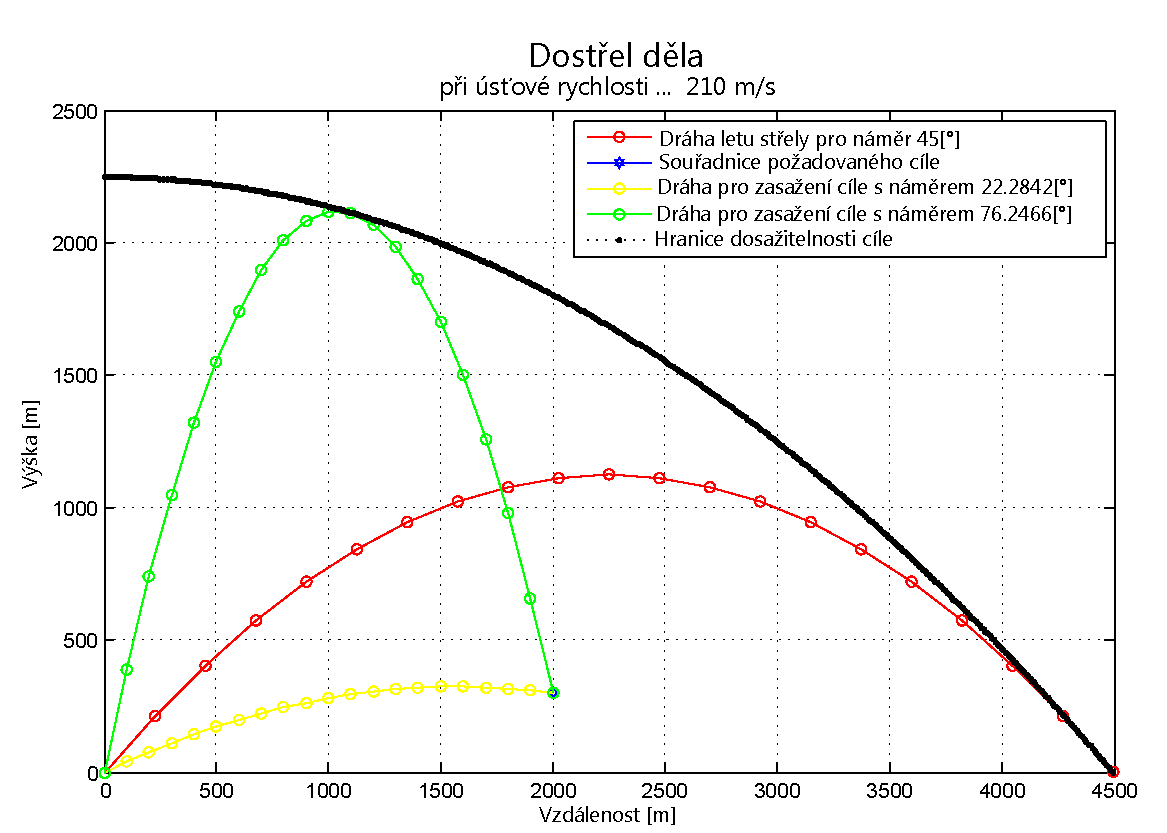
\includegraphics[width=\linewidth]{kinematika_delo_vakuum_matlab.pdf}
            \caption[Výpočet trajektorie projektilu]{Výpočet trajektorie projektilu ve vakuu při
                     úsťové rychlosti $210 m/s$ pomocí sw
                     MATLAB\textsuperscript{\textregistered}.}
            \label{mech:fig_delo_matlab}
          \end{figure}
        \end{example}
        \newpage
        \begin{example}
          Kolo vagónu se valí po vodorovné kolejnici. Uvažujte bod, který je v počátečním okamžiku
          pod středem kola ve vzdálenosti, která může být menší, rovna nebo větší než vzdálenost
          středu kola od kolejnice.
          \begin{figure}[ht!]
            \centering
            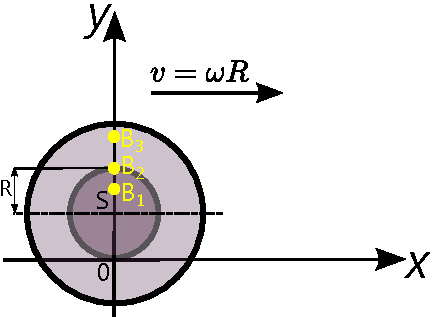
\includegraphics[scale=1]{trajectory_wheel_carriage.pdf}
            \caption{Kolo vagónu a tři možné polohy bodu}
            \label{mech:fig_wheel_1}
          \end{figure}
          \newline
          Určete  parametrické rovnice dráhy zvoleného bodu, složky rychlosti a její velikost,
          složky zrychlení a jeho velikost, tečné a normálové zrychlení a poloměr křivosti dráhy.
          \cite[p.~11]{Slavik}
          \newline
          \textbf{Řešení}: Obvodová rychlost v místě dotyku s kolejnicí je $v=\omega R$, což
          vzhledem k předpokladu o valení představuje posuvnou rychlost kola. Parametrické
          rovnice pro střed kola jsou pak
          \begin{align}\label{mech:eq_wheel_center}
            x_S &= \omega R t \\
            y_S &= R
          \end{align}
          Uvažovaný bod $B_3$ na obr. \ref{mech:fig_wheel_xy} je ve své nové pozici v čase $t_1$
          posunut vůči středu o vzdálenost $r\cdot\sin\omega t$ ve směru osy $x$ a o vzdálenost
          $r\cdot\cos\omega t$ ve směru osy $y$. Z obrázku \ref{mech:fig_wheel_xy} lze odvodit
          následující rovnice pro souřadnice libovolného bodu \emph{B} na kole vagónu.
          \begin{figure}[ht!]
            \centering
            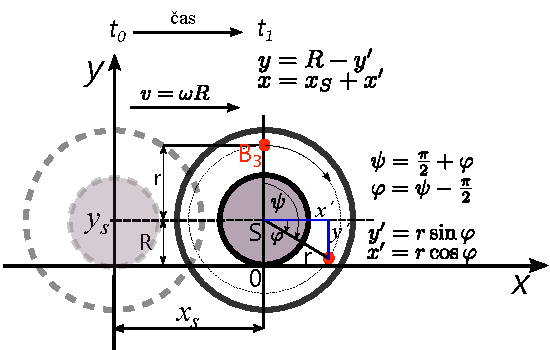
\includegraphics[scale=1.2]{trajectory_wheel_carriage_solve.pdf}
            \caption[Náčrt pro odvození rovnic pohybu bodu na kole vagónu]{Náčrt pro odvození
                     parametrických rovnic pohybu libovolně zvoleného bodu na kole vagónu}
            \label{mech:fig_wheel_xy}
          \end{figure}
                   
          \begin{minipage}[t]{0.5\textwidth}% first column
            \begin{itemize}
              \item ve směru osy x:                                        
              \begin{align*}
                x &= x_S + x'                        \\
                x &= x_S + r\cos(\psi-\frac{\pi}{2}) \\
                x &= x_S + r\sin\psi                 \\
                x &= \omega R t + r\sin\omega t
              \end{align*}
              \end{itemize}  
          \end{minipage}%second column           
          \begin{minipage}[t]{0.5\textwidth}
           \begin{itemize}
              \item ve směru osy y: 
              \begin{align*}
                y &= y_S - y'                        \\
                y &= y_S - r\sin(\psi-\frac{\pi}{2}) \\
                y &= y_S + r\cos\psi                 \\
                y &= R + r\cos\omega t
              \end{align*}
            \end{itemize}                 
          \end{minipage}
          % VERY important here is that there is no space between the /end{minipage} and the next
          %\begin{minipage} (obviously not counting comments). Otherwise LaTeX will not render the
          % columns side by side. 
          takže, parametrické rovnice dráhy mají tvar \textbf{cykloidy} viz
          \ref{mech_eq_cykloida}.
          \begin{align}\label{mech_eq_cykloida}
            x &= \omega R t + r\sin\omega t\\
            y &= R + r\cos\omega t
          \end{align}
          \begin{itemize}
            \item Složky rychlosti:
              \begin{align}\label{mech_eq_cykloida_v}
               v_x &= \frac{dx}{dt} = \omega R + r\omega\cos\omega t \nonumber \\
               v_y &= \frac{dy}{dt} = -r\omega\sin\omega t           \nonumber \\
               v   &= \sqrt{v_x^2 + v_y^2}= \omega\sqrt{R^2 + 2Rr\cos\omega t + r^2}
              \end{align}
            \item Složky zrychlení:
              \begin{align}\label{mech_eq_cykloida_a}
                a_x &= \frac{dv_x}{dt} = -r\omega^2\sin\omega t \\
                a_y &= \frac{dv_y}{dt} = -r\omega^2\cos\omega t \\
                a   &= \sqrt{a_x^2 + a_y^2}= r\omega^2\sqrt{\sin^2\omega t + 
                       \cos^2\omega t} = r\omega^2
              \end{align}
              Tento výsledek je superpozicí rovnoměrného kruhového a rovnoměrného přímočarého
              pohybu.
            \item Tečné zrychlení dostaneme derivací velikosti rychlosti
              \begin{align}\label{mech_eq_cykloida_at}
                a_t &= \frac{dv}{dt} = \omega\cdot\frac{1}{2\sqrt{R^2 + 2Rr\cos\omega t + r^2}}
                       \cdot(-1)\cdot2Rr\omega\sin\omega t  \\
                a_t &= \frac{r\omega^2\cdot|R\cos\omega t-r|}{\sqrt{R^2 + 2Rr\cos\omega t + r^2}}
              \end{align}
            \item Normálové zrychlení získáme užitím Pythagorovy věty
              \begin{align*}
                a_n &= \sqrt{a^2 - a_t^2} \\
                a_n &= \sqrt{(r\omega^2)^2-\left(
                       \frac{Rr\omega^2\sin\omega t}
                            {\sqrt{R^2 + 2Rr\cos\omega t + r^2}}\right)^2}                      \\
                a_n &= \frac{r\omega^2|R\cos\omega t - r|}{\sqrt{R^2 + 2Rr\cos\omega t + r^2}}
              \end{align*}
            \item Poloměr křivosti $R_0$ dostaneme ze vztahu $a_n=\frac{v^2}{R_0}$:
              \begin{align*}\label{mech:eq_cykloida_R0}
                  R_0 &=  \cfrac{\omega^2(R^2 + 2Rr\cos\omega t + r^2)}
                         {\cfrac{r\omega^2|R\cos\omega t - r|}
                         {\sqrt{R^2 + 2Rr\cos\omega t + r^2}}}                                  \\
                  R_0 &=  \frac{(R^2 + 2Rr\cos\omega t + r^2)^
                         {\frac{3}{2}}}{|Rr\cos\omega t - r^2|}
              \end{align*}
              Poloměr křivosti není roven vzdálenosti od středu kola r: drahou bodu není
              kružnice, nýbrž cykloida (viz obr. \ref{mech:fig_wheel_cycloid}).
          \end{itemize}
          \begin{align*}
            (x - \omega R t)^2            &= r^2\sin^2\omega t                          \\
            (y-R)^2                       &= r^2\cos\omega t                            \\
            (x - \omega R t)^2 + (y-R)^2  &= r^2\sin^2\omega t + r^2\cos\omega t        \\
            (x - \omega R t)^2 + (y-R)^2  &= r^2 \quad \text{kde}\; t = 
                                             \frac{1}{\omega}\arccos\frac{y-R}{r}       \\
            \left(x - R\arccos\frac{y-R}{r}\right)^2 + (y-R)^2  &= r^2
          \end{align*}
          \begin{figure}[ht!]
            \centering
            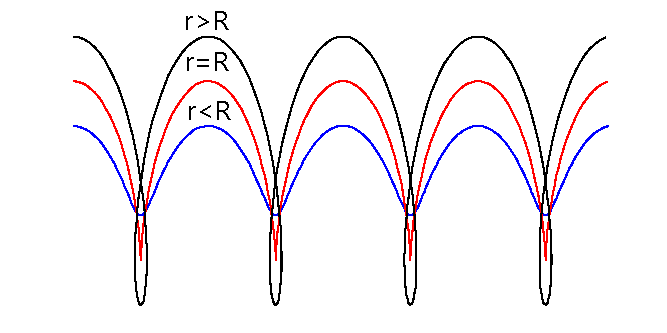
\includegraphics[width=0.9\linewidth]{trajectory_wheel_cycloid.pdf}
            \caption[Cykloida]{Cykloida: pro $B_2\ldots r=R$ je cykloida prostá; $B_3\ldots r>R$
                               cykloida prodloužená; $B_1\ldots r<R$ cykloida zkrácená;
                               \texttt{[cykloida.m]} }
            \label{mech:fig_wheel_cycloid}
          \end{figure}
        \end{example}
          
    \subsubsection{Skládání harmonických pohybů v kolmých směrech}
      Zmíníme se ještě o skládání \textbf{harmonických pohybů v kolmých smě\-rech}. Sklá\-dá\-me-li dva 
      takové pohyby o stejné úhlové frekvenci, bude výsledný pohyb probíhat po trajektorii dané parametrický 
      jako
      \begin{equation}\label{mech:eq_lissaujous1}
          x=A\sin(\omega t+\varphi_{01}),\qquad y=B\sin(\omega t +\varphi_{02})
      \end{equation}
      Výsledný pohyb vytváří zajímavé geometrické tvary známé pod názvem Lissajousovy obrazce. Jejich vzhled 
      závisí na poměru frekvencí a na fázovém úhlu \cite{Okrouhlik}.

      Označíme fázi kmitů ve směru $x$ jako $\omega t+\varphi_{01} = \varphi$, rozdíl fází obou kmitů jako 
      $\varphi_{02}-\varphi_{01} =\delta$. Dále vyloučíme z parametrických rovnic čas. K tomu cíli vyjádříme 
      $sin\varphi$ a $cos\varphi$ pomocí veličin na čase nezávisejících a použijeme známý vztah $sin^2\varphi 
      + cos^2\varphi = 1$. Máme
      \begin{equation}\label{mech:eq_lissajous2}
          \sin\varphi=\frac{x}{A}, \qquad 
          \sin(\varphi+\delta)=\sin\varphi\cos\delta+\cos\varphi\sin\delta=\frac{y}{B}
      \end{equation}
      odkud
      \begin{equation}\label{mech:eq_lissajous3}
          \cos\varphi=\frac{1}{\sin\delta}\left(\frac{y}{B}-\frac{x}{A}\cos\delta\right)
      \end{equation}
      Sečteme-li nyní $sin^2\varphi$ a $cos^2\varphi$, dostaneme rovnici trajektorie
      \begin{equation}\label{mech:eq_lissajous4}
          \frac{x^2}{A^2}+\frac{y^2}{B^2}-\frac{2xy}{AB}\cos\delta=\sin^2\delta
      \end{equation}
      V závislosti na $\delta$ může tato rovnice odpovídat rovnici \emph{úsečky}, nebo \emph{elipsy}. Je-li 
      $\delta = n\pi$, probíhají kmity po úsečce, jejíž přímka má směrnici $k = \pm\frac{B}{A}$, je-li 
      $\delta = \left(n + \frac{1}{2}\right)\pi$, je trajektorií
      elipsa
      \begin{equation}\label{mech:eq_lissajous5}
          \frac{x^2}{A^2}+\frac{y^2}{B^2}=1
      \end{equation}

      Jsou-li amplitudy obou pohybů stejné, přejde pro $\delta = \left(n+\frac{1}{2}\right)\pi$ elipsa v 
      kružnici. S uvedeným skládáním dvou kolmých pohybů o stejných frekvencích se setkáváme nejen v 
      mechanice, ale například i v elektromagnetismu a optice při studiu polarizace světla. Výsledné 
      trajektorie získané pomocí počítače jsou na obr. \ref{mech:fig_lissajous_1} a obr. 
      \ref{mech:fig_lissajous_2} \cite{Stoll}.

      \begin{figure*}
        \centering
        \subfloat[$A=B$ a $\omega_1=\omega_2$.]{\label{mech:fig_lissajous_1}
           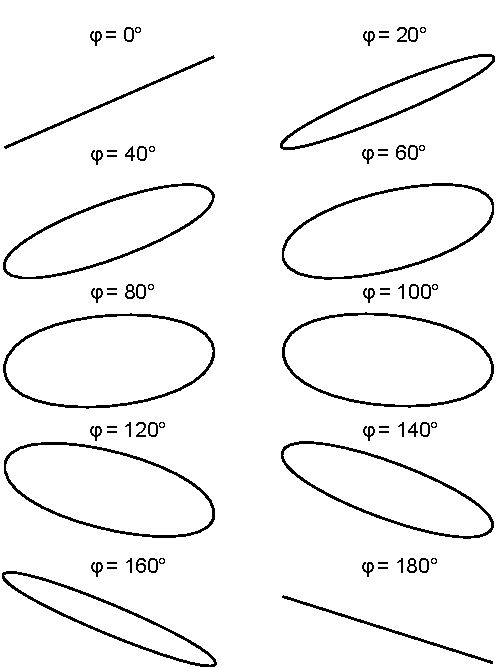
\includegraphics[width=0.4\textwidth]{lissajous_1.pdf}}
        \subfloat[$A=B$ a $\frac{\omega_1}{\omega_2}=\frac{2}{3}$.]{\label{mech:fig_lissajous_2}
           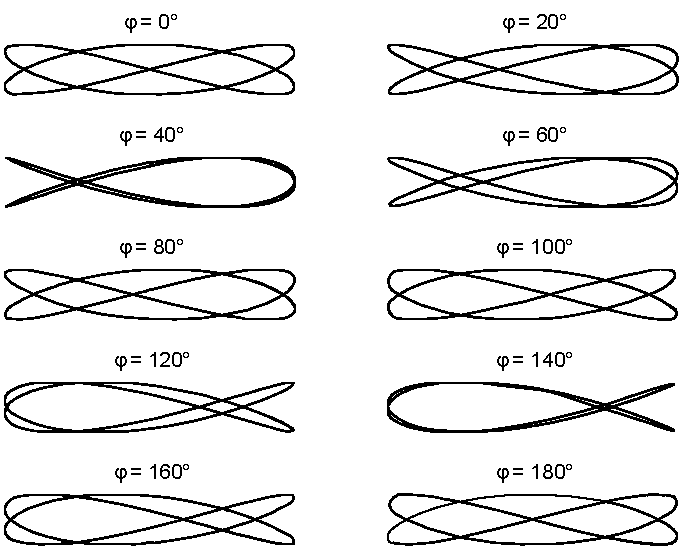
\includegraphics[width=0.6\textwidth]{lissajous_2.pdf}}
        \caption[Skládání harm. pohybů v kolmých směrech]{Trajektorie harmonických pohybů
                 $x=A\sin(\omega_1 t)$ a $y=B\sin(\omega_2 t+\varphi)$ v kolmých směrech}
        \label{mech:fig_lissajous_obrazce}
      \end{figure*}

      Jsou-li úhlové frekvence kolmých pohybů různé, vznikají složité tzv. \textbf{Lissajousovy obrazce} viz 
      \ref{mech:fig_lissajous_2}. Program ukazuje, jak se projevuje změna fázového úhlu při daném poměru 
      frekvencí obou pohybů.

      %---------------------------------------------------------------
        \lstinputlisting{../src/MECH/img/Lissajous.m}
        \begin{lstlisting}[caption=\texttt{Lissajous.m}vykreslí skládání harmonických pohybů v kolmých 
        směrech.]
        \end{lstlisting}
      %---------------------------------------------------------------
